%----------------------------------------------------------------------------------------
%	Packages
%----------------------------------------------------------------------------------------

\documentclass[11pt]{diazessay} % Font size (can be 10pt, 11pt or 12pt)

%----------------------------------------------------------------------------------------
%	Title
%----------------------------------------------------------------------------------------

\title{\textbf{Motion of Three Bodies in Space}} % Title and subtitle
\author{\textbf{Taylor Larrechea} \\ \textit{Colorado Mesa University}} % Author and institution
\date{October 31, 2019} %Date

%----------------------------------------------------------------------------------------
%	Begin Document
%----------------------------------------------------------------------------------------

\begin{document}
\maketitle % Print the title section

%----------------------------------------------------------------------------------------
%	Abstract
%----------------------------------------------------------------------------------------

\begin{abstract}
Come join us in WS 203 this Halloween at 12:30 PM for a seminar on the motion of three bodies in space! Using Newtonian Gravitation we will cover the dynamics of binary celestial body systems up to ternary star systems. Numerical methods are covered for how these differential equations were solved in order to plot the motion of these bodies. As always, coffee and cookies will be served for your liking.
\end{abstract}

%----------------------------------------------------------------------------------------
%	Document
%----------------------------------------------------------------------------------------
\begin{center}
\begin{figure}[htpb]
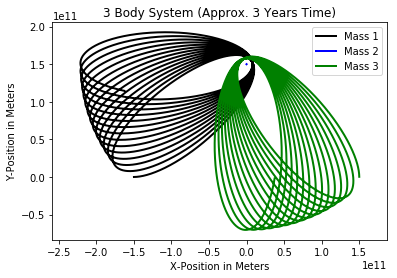
\includegraphics[width=1.00\linewidth]{Figures/3BodyDynamics.png}
\end{figure}
\end{center}
\end{document}

%----------------------------------------------------------------------------------------
%	Comment Headers
%----------------------------------------------------------------------------------------

%----------------------------------------------------------------------------------------
%	
%----------------------------------------------------------------------------------------